% Made up for the tikra benchmark.
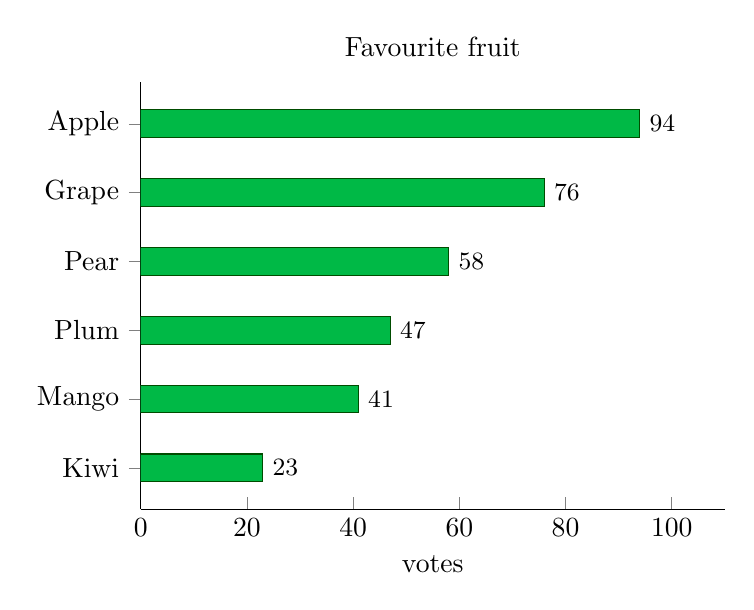
\begin{tikzpicture}
\begin{axis}[xbar, bar width=10pt, xmin=0, xmax=110, width=9cm, height=7cm,
    symbolic y coords={Kiwi, Mango, Plum, Pear, Grape, Apple}, ytick=data,
    xlabel={votes}, title={Favourite fruit}, nodes near coords, nodes near coords align=horizontal,
    every node near coord/.append style={font=\small}, axis x line*=bottom, axis y line*=left,
    enlarge y limits=0.12]
  \addplot[fill=green!45!teal, draw=green!30!black] coordinates
    {(23,Kiwi) (41,Mango) (47,Plum) (58,Pear) (76,Grape) (94,Apple)};
\end{axis}
\end{tikzpicture}
